\documentclass{article}
\usepackage{graphicx} % Required for inserting images
\usepackage[utf8]{inputenc}
\usepackage[T1]{fontenc}
\usepackage{amsmath}
\usepackage{tikz}
\def\abc#1{\begingroup\escapechar-1 \expandafter\string\csname#1\endcsname\endgroup}
\usepackage{ragged2e} % package pour justifier le texte
\usepackage{hyperref}

\title{Rapport de projet}
\author{PEREIRA David, GENEIX Lilian Groupe01}
\date{April 2023}


\begin{document}



\maketitle

\href{https://gitlab.isima.fr/dapereira3/jeu-du-pendu}{Lien vers le projet}


\section{Introduction}

Le projet consiste en la création d'un jeu du pendu en Python, avec l'ajout d'une interface graphique à l'aide de la bibliothèque Pygame. Le projet est organisé en plusieurs fonctions obligatoires, telles que la demande de proposition, la création d'un dictionnaire de fréquences de lettres et la génération aléatoire d'une liste de lettres triées par fréquence décroissante. Après la finalisation des fonctions principales, une interface graphique a été ajoutée, avec différents thèmes pour des niveaux de difficulté croissants. Le programme principal est un menu qui permet à l'utilisateur de sélectionner le mode de jeu souhaité. Le code est structuré en architecture de plugins, avec des fichiers JSON pour stocker les plugins et les données associées. Des patterns de conception tels que le pattern strategy, le pattern factory et parfois le pattern MVC ont été utilisés, ainsi que des concepts de POO tels que les classes et l'héritage. En outre, le typage des variables a été utilisé pour améliorer la lisibilité du code.

\section{Organisation pendant le semestre}

Au début du projet, nous avons créé la structure de chaque fonction obligatoire dans un fichier unique pour chacune. Ensuite, nous avons décidé qui se chargerait de chaque fonction, ce qui a été fait assez rapidement. Une fois les fonctions obligatoires terminées, nous avons listé toutes les tâches à effectuer pour l'interface graphique. Une fois cette organisation terminée, David s'est occupé de créer la structure de plugin, ce qui a permis d'ajouter des fonctionnalités facilement. De ce fait, de nombreuses fonctionnalités ont été ajoutées des deux côtés. Une fois les fonctionnalités principales terminées, tout le code a été documenté. Après la finalisation de l'interface, nous avons révisé toutes les fonctions obligatoires pour corriger d'éventuelles erreurs et avons finalement créé le menu principal.

\section{Les fonction obligatoires}

\subsection{La fonction demander proposition}

La fonction \verb|demander proposition| est une fonction qui demande à
l'utilisateur une lettre unique qui n'a pas été déjà entrée. Elle prend en entrée la liste \verb|deja_dit|, qui contient les lettres déjà entrées par l'utilisateur. La première ligne de la fonction modifie la casse de tous les éléments dans \verb|deja_dit| en majuscules, afin d'éviter des problèmes potentiels de casse plus tard dans la fonction. La deuxième ligne demande à l'utilisateur d'entrer une lettre, puis convertit cette lettre en majuscule.


Les 4 variables booléennes suivantes sont utilisées pour valider que la proposition de l'utilisateur est unique et valide:

\begin{itemize}
  \item \verb|is_unique_char| vérifie que la proposition est composée d'un seul caractère.
  \item \verb|is_in_deja_dit| vérifie que la proposition n'a pas déjà été entrée.
  \item \verb|is_in_ascii| vérifie que la proposition appartient à l'alphabet ASCII.
  \item \verb|is_letter| vérifie que la proposition est une lettre majuscule de l'alphabet.
\end{itemize}

Si l'une des conditions n'est pas satisfaite, alors cette même fonction est appelée de manière récursive pour demander une nouvelle proposition valide.

Si toutes les conditions sont satisfaites, alors la proposition valide est renvoyée.

Nous vons utiliser cette fonction dans \abc{partie_humain} ainsi que \abc{partie_humain_alea}, elle est utilisé pour récupérer les lettres donners par l'utilisateur et ainsi vérifie si elles sont valide en prenant les 4 booléens dit plus tôt.

\subsection{La fonction \abc{dico_frequence}}

La fonction \verb|dico_frequence| crée un dictionnaire qui contient la fréquence d'apparition de chaque lettre dans un fichier donné. La première ligne de la fonction appelle une autre fonction appelée \verb|importer_mots| qui importe les mots du fichier spécifié. La deuxième ligne convertit la liste des mots en une seule chaîne de caractères, ce qui permet d'éviter une boucle supplémentaire plus tard dans le code. La troisième ligne initialise un dictionnaire vide appelé \verb|frequence_dict| pour stocker les fréquences de chaque lettre. La boucle \verb|for| parcourt chaque caractère de la chaîne de caractères résultant de la deuxième ligne. Pour chaque lettre, elle vérifie si elle est déjà présente dans le dictionnaire \verb|frequence_dict|. Dans l'affirmative, elle incrémente simplement sa valeur associée. Dans le cas contraire, elle ajoute cette lettre au dictionnaire avec une valeur initiale de 1. Finalement, la fonction renvoie le dictionnaire \verb|frequence_dict| contenant les fréquences de
chaque lettre dans le fichier donné.
Nous avons utiliser cette fonction dans \abc{call_partie_auto}, elle a 1 chance sur 3 d'être utiliser par l'IA lorsqu'il devine un mot. Un treshold est initialiser de 5 et toute lettres ayant un une valeur supérieur dans le dictionnaire seras mis dans une liste et utiliser dans \abc{partie_auto}

\newpage

\subsection{La fonction \abc{fabrique_liste_alea}}

La fonction \verb|fabrique_liste_alea| crée une liste de lettres triées par fréquence décroissante. La première ligne de la fonction appelle la fonction \verb|dico_frequence| pour obtenir un dictionnaire des fréquences de chaque lettre dans le fichier spécifié. La deuxième ligne initialise une liste vide appelée \verb|liste|. La boucle \verb|while| parcourt le dictionnaire \verb|dico| tant qu'il n'est pas vide. Pour chaque itération, elle appelle une autre fonction appelée \verb|lettre_la_plus_frequente| qui renvoie la lettre la plus fréquente dans le dictionnaire. Elle ajoute ensuite cette lettre à la fin de la liste \verb|liste|. Enfin, elle supprime cette lettre du dictionnaire pour éviter qu'elle ne soit sélectionnée à nouveau. Finalement, lorsque toutes les lettres ont été sélectionnées et ajoutées à la liste, celle-ci est renvoyée triée par ordre décroissant de fréquence.
Nous avons utiliser cette fonction dans la fonction \abc{call_partie_auto}, elle créer la liste qui est utiliser dans \abc{partie_auto} pour deviner le mot mystére de maniére plus optimale par rapport a la bases de données utiliser pour choisir un mot.

\section{Les extentions}
\subsection{Plugin et interface graphique}

Nous avons ajouter une extention principale qui est une interface graphique qui utilise la librairie Pygame. 

\begin{itemize}
    \item En quoi elle consiste ? Nous avons créé une nouvelle version du jeu du pendu en utilisant une interface graphique, comme mentionné précédemment. L'objectif était de rendre le jeu plus efficace et plus agréable en permettant aux joueurs d'utiliser leur clavier et de voir en temps réel l'avancement du mot et le nombre de vies restantes, affiché en haut à droite de l'écran. Bien que le jeu comporte des monstres, ceux-ci ne sont présents que pour des raisons esthétiques. Toutefois, à chaque fois qu'une vie est perdue, un monstre meurt et si tous les monstres meurent, la partie est terminée et nous avons perdu. Si vous jouez plusieurs fois, vous remarquerez qu'il y a différents thèmes disponibles, représentant différents niveaux de difficulté. Le thème "prairie" est considéré comme facile, avec un mot de cinq lettres, tandis que le thème "cave" est de niveau moyen, avec un mot de dix lettres. Enfin, le dernier thème, "mode difficile", est le plus difficile, avec un mot de quinze lettres. 
    \item Nous avons incorporé la fonctionnalité de lancer l'interface graphique depuis le menu principal pour faciliter son utilisation. Une fois que le programme est lancé, il suffit de sélectionner le mode graphique et c'est tout. Une fois dans le jeu, vous verrez trois boutons: le premier pour démarrer le jeu, le deuxième pour accéder au menu (cependant, il ne fonctionne pas) et le dernier pour quitter le jeu. Lorsque vous jouez, vous devrez appuyer sur une touche de votre clavier pour tester la lettre. Si la lettre est correcte, elle s'affiche à l'écran, sinon vous perdez une vie et un monstre meurt. Si vous gagnez ou perdez, un écran s'affichera et si vous souhaitez recommencer, vous devrez relancer le programme.
    \item Tout d'abord, la structure globale du projet est basée sur une architecture de plugins. Ainsi, tout ce qui est affiché à l'écran est indépendant et n'est pas directement lié au jeu. Tout est géré grâce à deux fichiers JSON : le premier stocke tous les plugins et le second stocke les données nécessaires à certains plugins. Cette approche a été choisie pour éviter les conflits sur le fichier principal et pour éviter qu'une boucle de jeu ne soit une énorme fonction de 300 lignes. De plus, plusieurs design patterns ont été utilisés dans le code, tels que le pattern strategy, le pattern factory, parfois un pattern MVC, etc. Bien sûr, des concepts de POO ont été utilisés, tels que les classes et l'héritage, ainsi que d'autres fonctionnalités propres à Python, comme les dataclass. Dans l'ensemble du projet, l'utilisation du typage des variables est visible pour rendre le code plus lisible.
\end{itemize}
\subsection{Neural Network}
Cette extension est une implémentation d'un réseau de neurones artificiels pour le jeu du pendu en devinant les lettres d'un mot donnée.

Le programme définit le nombre de noeuds d'entrée, de sortie et cachés du réseau de neurones, ainsi que la fonction d'activation et sa dérivée.La classe 'NeuralNetwork' est ensuite définie, avec des méthodes pour initialiser les poids aléatoires, effectuer la propagation avant, l'entrainement et la prédiction.

Le programme utilise la fonction sigmoïde comme fonction d'activation pour les neurones, ce qui permet de modéliser la non-linéarité de la relation entre les entrées et les sorties du réseau de neurones.
\begin{figure}[h]
\centering
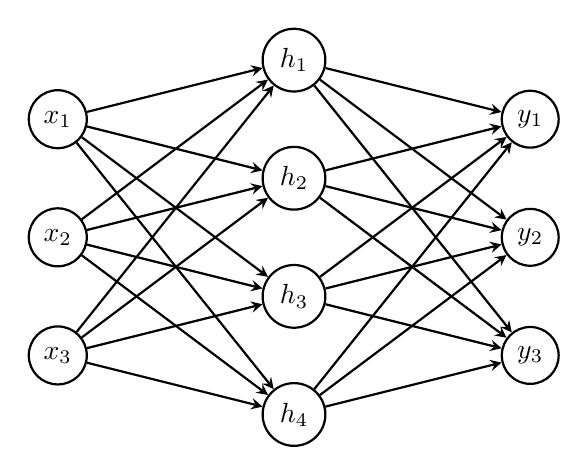
\begin{tikzpicture}[x=1.5cm, y=1.5cm, >=stealth]

% Les nœuds d'entrée (inputs)
\foreach \i in {1,...,3}
\node[circle, draw=black, thick, minimum size=0.5cm] (I\i) at (0,2-\i) {$x_\i$};

% Les nœuds de la couche cachée (hidden layer)
\foreach \h [count=\hi] in {1,...,4}
\node[circle, draw=black, thick, minimum size=0.5cm] (H\hi) at (2,2.5-\h) {$h_\h$};

% Les nœuds de sortie (output)
\foreach \o [count=\oi] in {1,...,3}
\node[circle, draw=black, thick, minimum size=0.5cm] (O\oi) at (4,2-\oi) {$y_\o$};

% Les connexions entre l'entrée et la couche cachée
\foreach \i in {1,...,3}
\foreach \h in {1,...,4}
\draw[->, thick] (I\i) -- (H\h);

% Les connexions entre la couche cachée et la sortie
\foreach \h in {1,...,4}
\foreach \o in {1,...,3}
\draw[->, thick] (H\h) -- (O\o);


\end{tikzpicture}
\caption{Exemple d'un réseau de neurones.}
\end{figure}

\begin{figure}[h]
\centering
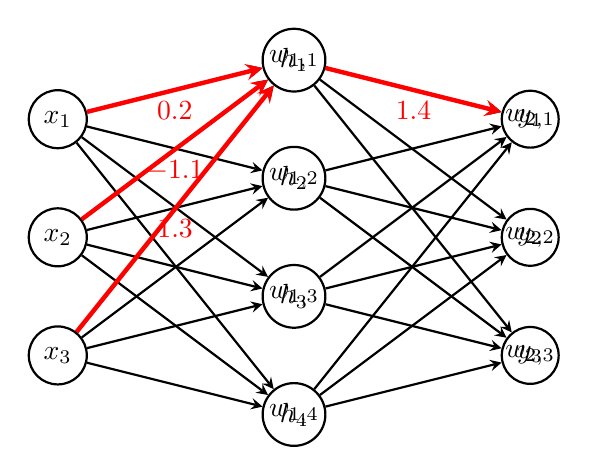
\begin{tikzpicture}[x=1.5cm, y=1.5cm, >=stealth]

% Les nœuds d'entrée (inputs)
\foreach \i in {1,...,3}
\node[circle, draw=black, thick, minimum size=0.5cm] (I\i) at (0,2-\i) {$x_\i$};

% Les nœuds de la couche cachée (hidden layer)
\foreach \h [count=\hi] in {1,...,4}
\node[circle, draw=black, thick, minimum size=0.5cm] (H\hi) at (2,2.5-\h) {$h_\h$};

% Les nœuds de sortie (output)
\foreach \o [count=\oi] in {1,...,3}
\node[circle, draw=black, thick, minimum size=0.5cm] (O\oi) at (4,2-\oi) {$y_\o$};

% Les connexions entre l'entrée et la couche cachée
\foreach \i in {1,...,3}
\foreach \h in {1,...,4}
\draw[->, thick] (I\i) -- (H\h);

% Les connexions entre la couche cachée et la sortie
\foreach \h in {1,...,4}
\foreach \o in {1,...,3}
\draw[->, thick] (H\h) -- (O\o);

% Les poids
\node[above of=H1, yshift=-1cm] {$w_{1,1}$};
\node[above of=H2, yshift=-1cm] {$w_{1,2}$};
\node[above of=H3, yshift=-1cm] {$w_{1,3}$};
\node[above of=H4, yshift=-1cm] {$w_{1,4}$};
\node[above of=O1, yshift=-1cm] {$w_{2,1}$};
\node[above of=O2, yshift=-1cm] {$w_{2,2}$};
\node[above of=O3, yshift=-1cm] {$w_{2,3}$};

% Flèche d'exemple
\draw[->, ultra thick, red] (I1) -- (H1) node[midway, below] {$0.2$};
\draw[->, ultra thick, red] (I2) -- (H1) node[midway, below] {$-1.1$};
\draw[->, ultra thick, red] (I3) -- (H1) node[midway, below] {$1.3$};
\draw[->, ultra thick, red] (H1) -- (O1) node[midway, below] {$1.4$};

\end{tikzpicture}
\caption{Exemple de poids dans un réseau de neurones.}
\end{figure}


Cette figure montre un exemple de poids dans un réseau de neurones. Le réseau de neurones est constitué d'une couche d'entrée avec trois nœuds (inputs), d'une couche cachée avec quatre nœuds (hidden layer) et d'une couche de sortie avec trois nœuds (output). Les connexions entre les nœuds sont représentées par des flèches, qui indiquent le sens du flux d'informations dans le réseau. Les poids des connexions sont indiqués près de chaque flèche.

Dans cet exemple, la flèche rouge indique un exemple de calcul de poids. Le nœud d'entrée $x_1$ a un poids de $0.2$ avec le nœud caché $h_1$, le nœud d'entrée $x_2$ a un poids de $-1.1$ avec le nœud caché $h_1$, le nœud d'entrée $x_3$ a un poids de $1.3$ avec le nœud caché $h_1$, et le nœud caché $h_1$ a un poids de $1.4$ avec le nœud de sortie $y_1$. Ces poids sont utilisés pour calculer la sortie du réseau de neurones en prenant en compte les entrées et les poids associés à chaque connexion.

\begin{figure}[h]
\centering
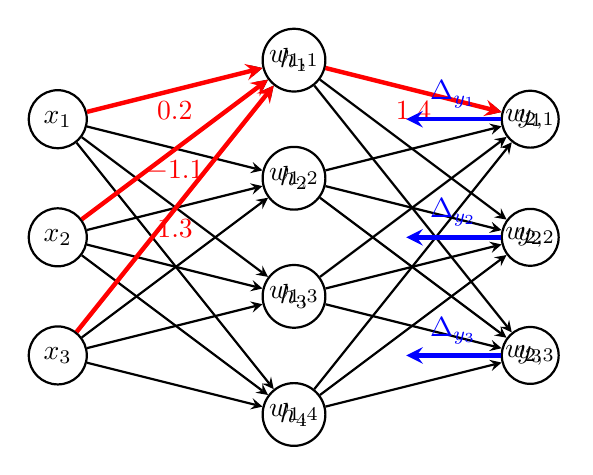
\begin{tikzpicture}[x=1.5cm, y=1.5cm, >=stealth]

% Les nœuds d'entrée (inputs)
\foreach \i in {1,...,3}
\node[circle, draw=black, thick, minimum size=0.5cm] (I\i) at (0,2-\i) {$x_\i$};

% Les nœuds de la couche cachée (hidden layer)
\foreach \h [count=\hi] in {1,...,4}
\node[circle, draw=black, thick, minimum size=0.5cm] (H\hi) at (2,2.5-\h) {$h_\h$};

% Les nœuds de sortie (output)
\foreach \o [count=\oi] in {1,...,3}
\node[circle, draw=black, thick, minimum size=0.5cm] (O\oi) at (4,2-\oi) {$y_\o$};

% Les connexions entre l'entrée et la couche cachée
\foreach \i in {1,...,3}
\foreach \h in {1,...,4}
\draw[->, thick] (I\i) -- (H\h);

% Les connexions entre la couche cachée et la sortie
\foreach \h in {1,...,4}
\foreach \o in {1,...,3}
\draw[->, thick] (H\h) -- (O\o);

% Les poids
\node[above of=H1, yshift=-1cm] {$w_{1,1}$};
\node[above of=H2, yshift=-1cm] {$w_{1,2}$};
\node[above of=H3, yshift=-1cm] {$w_{1,3}$};
\node[above of=H4, yshift=-1cm] {$w_{1,4}$};
\node[above of=O1, yshift=-1cm] {$w_{2,1}$};
\node[above of=O2, yshift=-1cm] {$w_{2,2}$};
\node[above of=O3, yshift=-1cm] {$w_{2,3}$};

% Flèche d'exemple
\draw[->, ultra thick, red] (I1) -- (H1) node[midway, below] {$0.2$};
\draw[->, ultra thick, red] (I2) -- (H1) node[midway, below] {$-1.1$};
\draw[->, ultra thick, red] (I3) -- (H1) node[midway, below] {$1.3$};
\draw[->, ultra thick, red] (H1) -- (O1) node[midway, below] {$1.4$};

% Les flèches de rétropropagation
\draw[->, ultra thick, blue] (O1.west) -- ++(-0.8,0) node[midway, above] {$\Delta_{y_1}$};
\draw[->, ultra thick, blue] (O2.west) -- ++(-0.8,0) node[midway, above] {$\Delta_{y_2}$};
\draw[->, ultra thick, blue] (O3.west) -- ++(-0.8,0) node[midway, above] {$\Delta_{y_3}$};

\end{tikzpicture}
\caption{Exemple rétropropagation.}
\end{figure}

Dans notre programme nous avons bien la fonction sigmoïd (def sigmoid), qui est utilisée comme une fonction d'activation dans le réseau de neurones. elle prend en entrée un nombre réel et renvoie un nombre compris entre 0 et 1, qui représente la probabilité que la sortie du neurone soit activée.

La dérivée de la fonction sigmoid (def \abc{sigmoid_derivative}) est nécessaire pour la rétropropagation du gradient, qui comme vue précédement permet d'ajuster le poids du réseau de neurones lors de l'apprentissage. \

Dans notre programme le réseau de neurones est défini comme une classe, lors de l'initialisation les poids des connexions synaptiques sont initialisés avec des valeurs aléatoires.

\abc{self.weights1 = np.random.rand(INPUT_NODES, HIDDEN_NODES)} \\

\abc{self.weights2 = np.random.rand(HIDDEN_NODES, OUTPUT_NODES)} \\ 

La méthode \abc{feed_forward} calcule la sortie de neurones pour une entrée donnée.Elle calcule d'abord la sortie de la couche cachée, puis la sortie de la couche de sortie. \\ 

La méthode train est utilisée pour entrainer le réseau de neurones sur un ensemble de données d'entraînement. elle utilise la méthode \abc{feed_forward} pour obtenir la sortie prédite du réseau de neurones pour chaque exemple d'entraîenement.Elle calcule ensuite l'erreur entre la sortie prédite et la sortie attendue, et utilise la rétropropagation du gradient pour ajuster les poids du réseau de neurones.Les ajustements sont calculés en multipliant l'erreur par la dérivée de la fonction d'acvtivation et en les transmettant de la couche de sortie à la couche cachée.Les poids sont ensuite mis à jour en utilisant les ajustements calculés. \\ 

La méthode predict permet d'utiliser le réseau de neurones entrînée pour fair une prédiction à partie d'un input X donnée. \\ 

Avec tout ceci nous pouvons créer les données d'entréer et de sortie, dans notre cas deux matrices X et y.Notre matrice X est remplie avec des zéros, à l'exception de la colonne correspondant à la lettre, qui est remplie avec un "1".La matrice y est remplie avec des zéros a l'exception de la ligne correspondant à l'index de la lettre, qui est remplie avec un "1". \\
\begin{center}
    
$X = \begin{bmatrix}
0 & 0 & 1 & 0 \\
0 & 1 & 0 & 0 \\
1 & 0 & 0 & 0 \\
0 & 0 & 0 & 1 
\end{bmatrix} 
y = \begin{bmatrix}
1 & 0 & 0 & 0 \\
0 & 1 & 0 & 0 \\
0 & 0 & 1 & 0 \\
0 & 0 & 0 & 1 
\end{bmatrix} $

\end{center}

Voici un exemple qui pourrais arriver pour un réseau de neurones avec 4 noeuds d'entrée et 4 noeuds de sortie si on lui donnée l'entrée "chat".
Ensuite le réseau de neurones est entrainer a l'aide de ces données qui sont séparés en vecteur de taille 4, il y a ensuite un affinage de la précision à l'aide de la méthode \abc{feeed_forward} et la rétropropagation.L'algorithme continue jusqu'a que le nombre d'itérations spécifique soit atteint.
Ensuite la programme 'predict' une lettre (l'indice du neurone ayant la sortie la plus élevée. Par exemple le vecteur de sortie dans notre exemple pourrais être [0.24,0.34,0.53,0.29], le troisiéme élément est le plus grand donc la lettre prédite sera 'a'.

\subsection{Extensions non utilisés}
Des essaies d'implémentation de différents gameplay, dans le fichier "Test Game", n'on pas aboutit.Tout d'abord une pluie de lettre tombant du haut de la fenêtre de jeu, le joueurs devant récupérer les lettres pour compléter le mot a deviner.
Puis cette extensions a était changer par un cube controler partiellement par le joueur pour ramasser les lettres manquants dans le mot a deviner.
Cette extensions est encore valable dans le fichier "Test Game" et peut être utiliser par sois même.
nous avons considére l'ajout de l'extension à notre projet. Cepedant, aprés une analyse plus approfondie, nous avons constaté que cette extension nécessiterait une réécriture importante de notre code existant.
Notre projet est assez avancé et comporte de nombreuses fonctionnalités complexes qui sont étroitement intégrées. Ajouter l'extension demandées signifierait que nous devrions changer les fondations de l'extension graphique et celle des Plugins.
Bien que cette extensions comporte un bon changement sur la maniére de jouer habituel nous avons décidé de ne pas l'ajouter mais elle peut quand même être utiliser a part.

\section{Structure du programme principal}

Le programme principal est un menu qui offre à l'utilisateur plusieurs options de jeu, y compris les fonctions obligatoires. Une fois le menu lancé, il suffit de choisir un numéro correspondant au mode de jeu souhaité.


\begin{thebibliography}{1}
\bibitem{playlist1}
\href{https://youtube.com/playlist?list=PLZHQObOWTQDNU6R1_67000Dx_ZCJB-3pi}{Neural Network by 3Blue1Brown}
\bibitem{Doc1}
\href{https://www.pygame.org/docs/}{Doc Pygame}
\bibitem{Doc2}
\href{https://numpy.org/doc/}{Doc numpy} 
\bibitem{website1}
\href{https://medium.datadriveninvestor.com/building-a-neural-network-from-scratch-using-python-1c143cb30f61}{Neural Network in Python} 
\end{thebibliography}

\end{document}

